\begin{frame}
\frametitle{CERN LHC}
\begin{center}
\begin{tikzpicture}
\node[anchor=south west,inner sep=0] at (0,0) {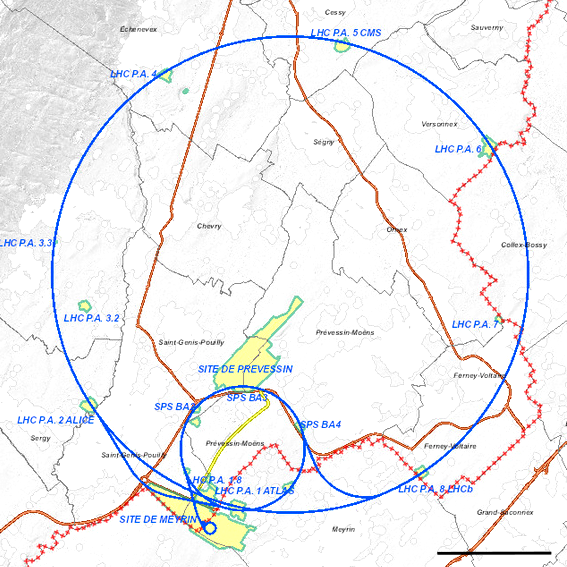
\includegraphics[scale=.35]{\PhDthesisdir/slides/LHC-CMS/LHC/CERN_LHC_map-scale_2km.png}};
\draw (6.125,.4) node {\SI{2}{\kilo\meter}};
\draw (2.95,.75) coordinate (LHCp1);
\draw (1.125,2) coordinate (LHCp2);
\draw (.65,4) coordinate (LHCp3);
\draw (1,3.2) coordinate (LHCp32);
\draw (2,6.1) coordinate (LHCp4);
\draw (4.25,6.45) coordinate (LHCp5);
\draw (6.05,5.15) coordinate (LHCp6);
\draw (6.15,3.125) coordinate (LHCp7);
\draw (5.15,1.15) coordinate (LHCp8);
\draw (LHCp1) coordinate (ATLAS);
\draw (LHCp2) coordinate (ALICE);
\draw (LHCp5) coordinate (CMS);
\draw (LHCp8) coordinate (LHCb);

%\foreach \coord in {1,2,3,4,5,6,7,8,32}{
%\fill[ltcolorred] (LHCp\coord) circle (3pt);
%}

%\draw [ultra thick, ltcolorred] (3.575,3.625) circle (2.95) ;
%\draw [ultra thick, ltcolorred] (3,1.475) circle (.75) ;
%\draw [ultra thick, ltcolorred] (2.6,.5) circle (.075) ;
%\fill [ltcolorred] (2.55,.55) circle (.05) ;
%\draw [ultra thick, ltcolorred] (2.5,.5) --+ (-60:.15) ;
\fill[ltcolorred] (CMS) circle (3pt);
\draw [ltcolorred4] (CMS) node [below] {\textbf{CMS}};
\fill[ltcolorred] (ATLAS) circle (3pt);
\draw [ltcolorred4] (ATLAS) node [above] {\textbf{ATLAS}};
\fill[ltcolorred] (ALICE) circle (3pt);
\draw [ltcolorred4] (ALICE) node [above right] {\textbf{ALICE}};
\fill[ltcolorred] (LHCb) circle (3pt);
\draw [ltcolorred4] (LHCb) node [below right] {\textbf{LHCb}};
\end{tikzpicture}
\end{center}
\end{frame}
